\documentclass{article}
\usepackage[spanish]{babel} 
\usepackage{multirow}
%\usepackage[latin1]{inputenc}
\usepackage[utf8]{inputenc}
\usepackage{graphicx}
\usepackage{lmodern}
\usepackage{listings}
\usepackage{color}
\usepackage{fancyhdr}
\usepackage{hyperref}
\usepackage[left=2.5 cm,right=2cm,top=2.5 cm,bottom=3cm]{geometry}
\usepackage{Sweave}
\begin{document}

\Sconcordance{concordance:CorrecionTest1.tex:CorrecionTest1.Rnw:%
1 12 1 1 0 132 1 1 3 36 0 1 2 2 1 1 3 3 0 1 1 3 0 1 2 11 1}

\pagestyle{fancy}
\renewcommand{\headrulewidth}{0pt}
\bigskip
\bigskip
{\setlength{\arrayrulewidth}{0.5mm}
\begin{tabular}{p{2 cm} | p{10
cm} p{3 cm}}
\multirow{3}{2cm}{\Large{
\includegraphics[width=1.9 cm]{unloja}}} 
&\Large{\textbf{UNIVERSIDAD}}&\multirow{3}{2cm}{\Large{
\includegraphics[width=3 cm]{logo13}}}\\

& \Large{\textbf{NACIONAL}}& \\
& \Large{\textbf{DE LOJA}}&\\
\end{tabular}
\bigskip
\bigskip
\begin{flushleft}
\raggedright{ 
  \small{\textit{\textbf{Area de la Energia, las Industrias y los Recursos Naturales No Renovables}}}
}
\thinspace
\rule{1\textwidth}{0.04cm} 
\thinspace
\raggedleft{ 
  \Large{\textsc{Carrera de Ingenieria en Sistemas}}}
\bigskip
\bigskip
\bigskip
\bigskip
\bigskip
\begin{center}
\begin{Huge}
\end{Huge}
\bigskip
\bigskip
\bigskip
\begin{LARGE}
\medskip
\textbf{CORRECCIÓN TEST DEL GRUPO A y GRUPO B}\\
\bigskip
\bigskip
\end{LARGE}
\textbf{Sexto A}\\
\bigskip
\end{center}
\bigskip
\bigskip
\begin{flushleft}
\textit{\textbf{Autores:}}
\begin{itemize}
\renewcommand{\labelitemi}{$\diamond$} 
\item \href{http://www.iralis.org/?q=node%2F10&paso=10&letra=P&id=5216/}{ECINF5216}
\item \href{http://www.iralis.org/?q=node%2F10&paso=10&letra=P&id=5186/}{ECINF5186}
\item \href{http://www.iralis.org/?q=node%2F10&paso=10&letra=P&id=5208/}{ECNIF5208}
\item \href{http://www.iralis.org/?q=node%2F10&paso=10&letra=P&id=7223/}{ECNIF7223}
\item \href{http://www.iralis.org/?q=node%2F10&paso=10&letra=P&id=5187/}{ECINF5187}
\item \href{http://www.iralis.org/?q=node%2F10&paso=10&letra=P&id=7317/}{ECINF7317}
\end{itemize}

\bigskip
\bigskip
\end{flushleft}
\thinspace
\bigskip
\begin{flushleft}
\textit{\textbf{Tutor:}}

\begin{itemize}
\renewcommand{\labelitemi}{$\diamond$} 
\item \href{http://www.iralis.org/?q=node%2F10&paso=10&letra=O&id=4796}{ECINF4796}
\end{itemize}
\bigskip
\bigskip
\end{flushleft}
\thinspace
\bigskip

\begin{center}
Loja - Ecuador \\
2015
\end{center}


\newpage

\begin{center}
\begin{Huge}
\textbf {CORRECCIÓN DEL TEST 1}\\
\end{Huge}
\end{center}
\begin{center}
\textbf {PARTE A}
\end{center}
\begin{itemize}
\item\textbf {Análisis textual de la parte A, del grupo A: }\\
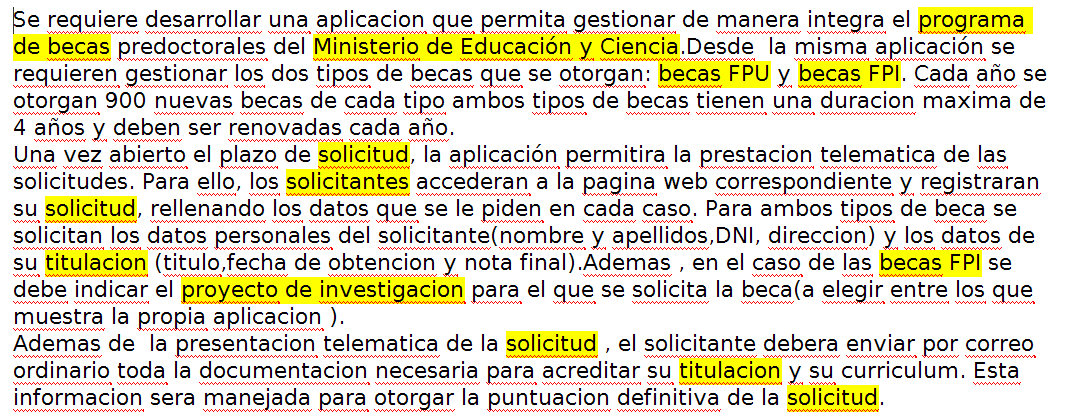
\includegraphics[width=16cm]{img/PARTEA1} \hspace{0.5cm}
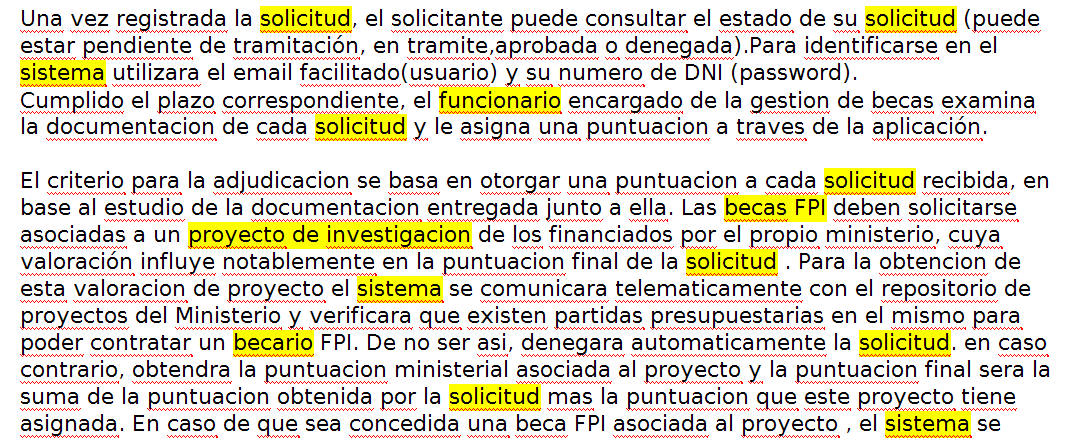
\includegraphics[width=16cm]{img/PARTEA2} \hspace{0.5cm}
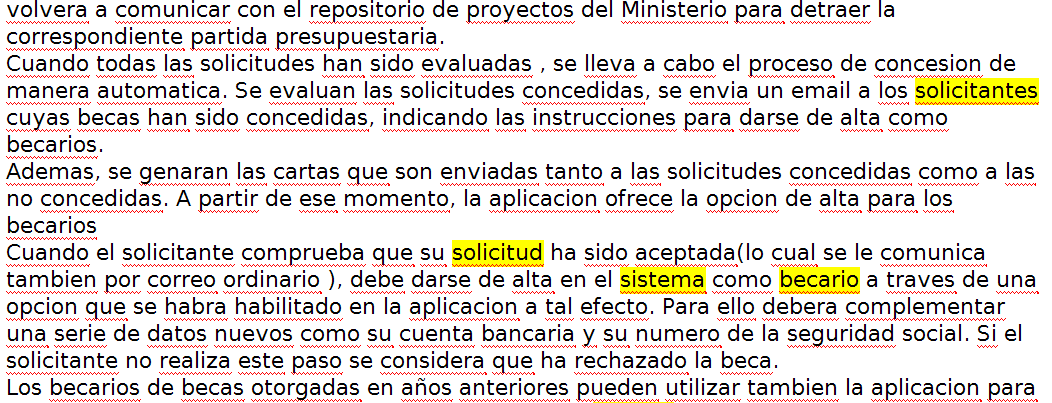
\includegraphics[width=16cm]{img/PARTEA3} \hspace{0.5cm}
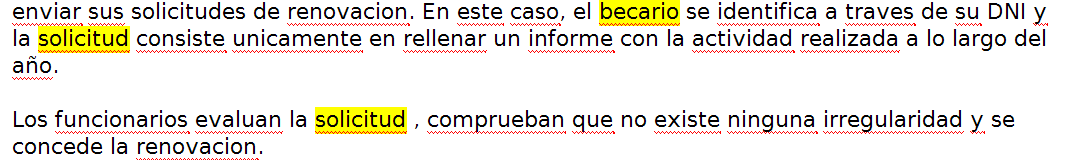
\includegraphics[width=16cm]{img/PARTEA4} \hspace{0.5cm}
\item\textbf {Clases candidatas: }\\
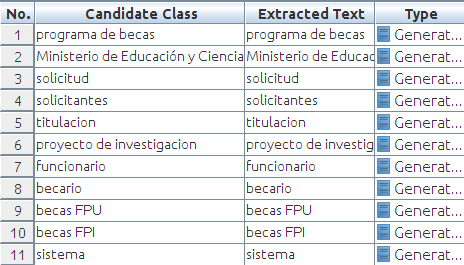
\includegraphics[width=12cm]{img/CLASES} \hspace{0.5cm}

\item\textbf {Diagrama de Clases Candidatas: }\\
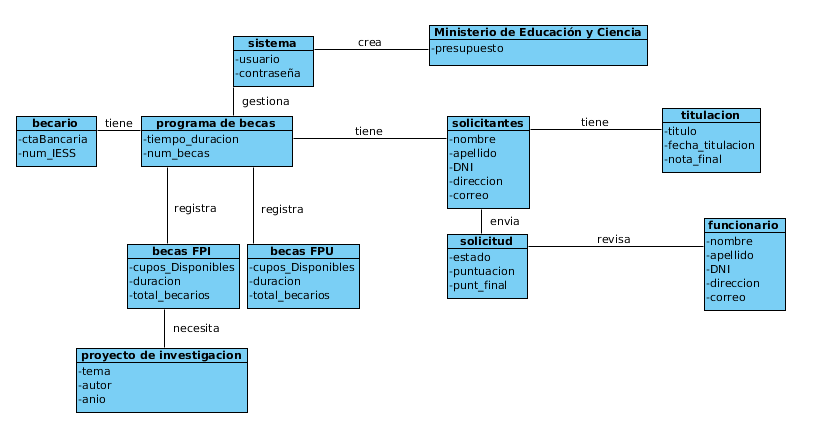
\includegraphics[width=16cm, height=11cm]{img/parteAmodelo} \hspace{0.5cm}
\newpage
\item\textbf {Análisis textual de la parte A, del grupo B: }\\
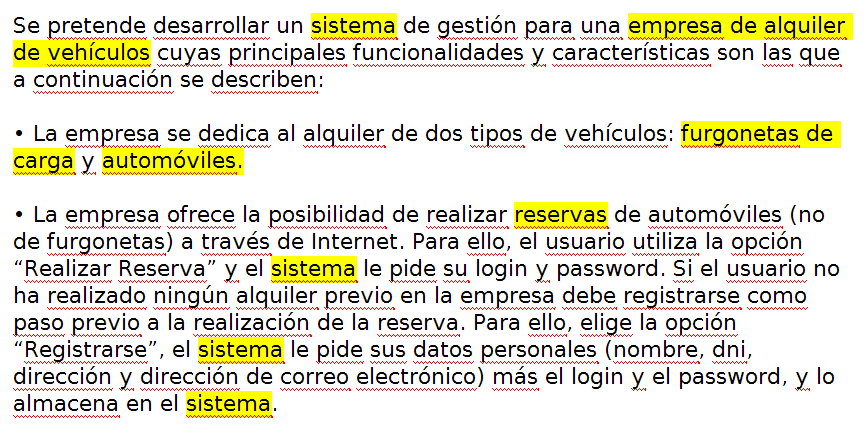
\includegraphics[width=16cm]{img/parteB1} \hspace{0.5cm}
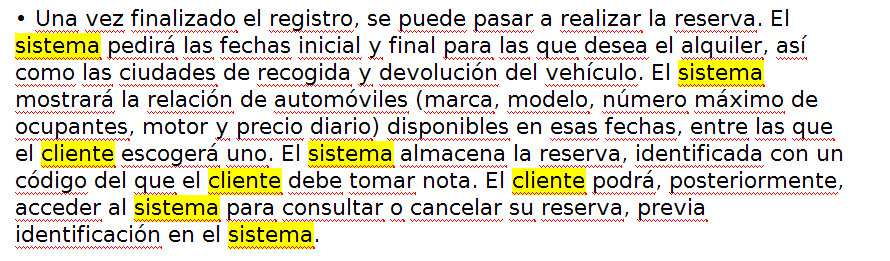
\includegraphics[width=16cm]{img/parteB2} \hspace{0.5cm}
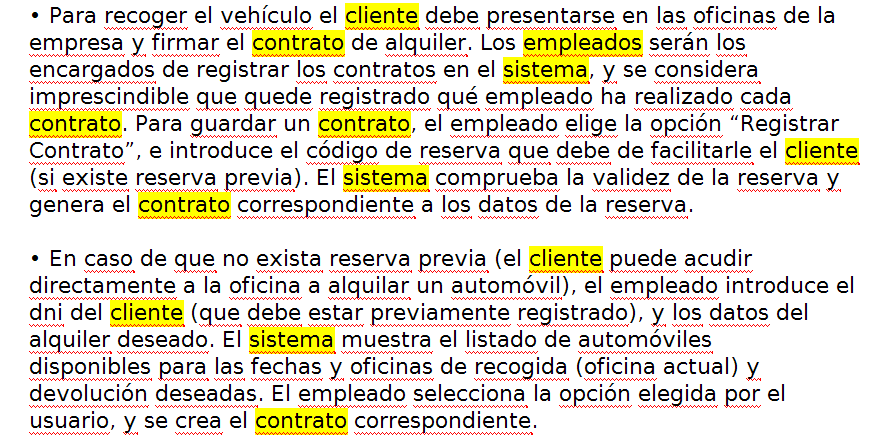
\includegraphics[width=16cm]{img/parteB3} \hspace{0.5cm}
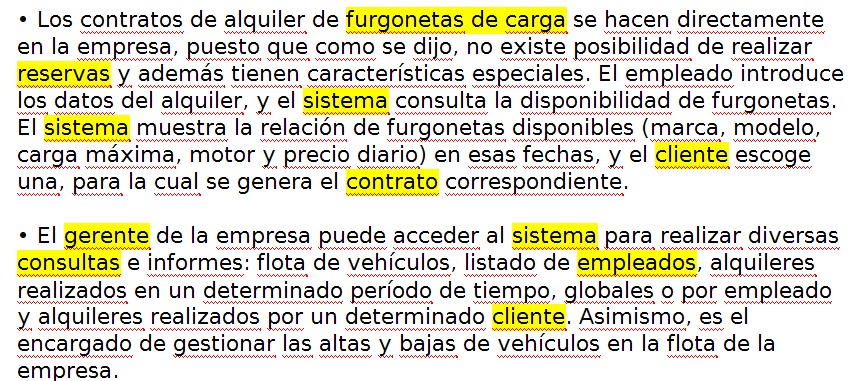
\includegraphics[width=16cm]{img/parteB4} \hspace{0.5cm}

\item\textbf {Clases candidatas: }\\
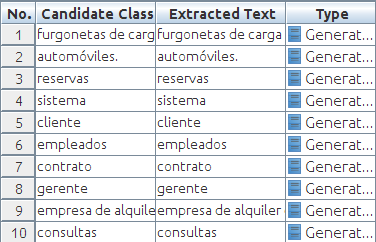
\includegraphics[width=14cm]{img/CLASESB} \hspace{0.5cm}
\newpage
\item\textbf {Diagrama de Clases Candidatas: }\\
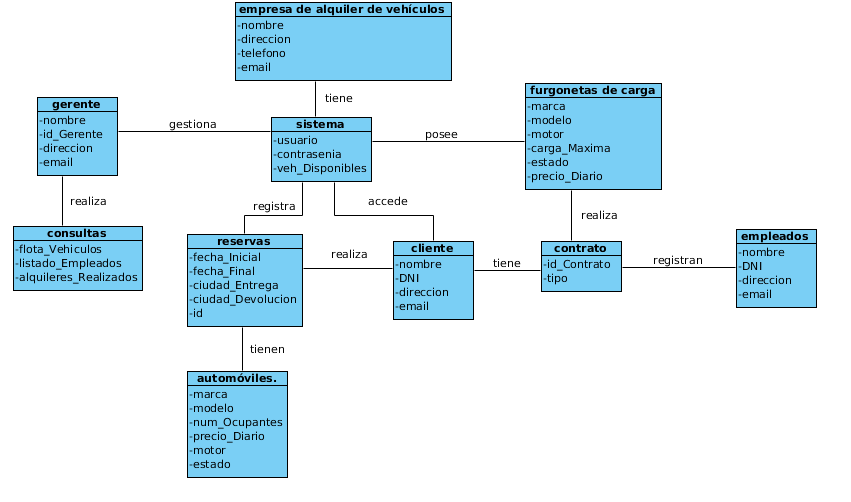
\includegraphics[width=18cm]{img/parteBmodelo} \hspace{0.5cm}\\
\begin{center}
\textbf {PARTE B}
\end{center}
\textbf{Desarrollar las siguientes actividades a partir del dataset Titanic (Data sets in package 'datasets'), y de la Ingeniería del Software:}\par

\textbf{1.¿Es aplicable la ingeniería de software cuando se elaboran webapps? Si es así, ¿cómo puede modificarse para que asimile las características únicas de éstas?}\par
Si es aplicable la ingenieria de software cuando se elaboran webapps ya que en la actualidad las webapps an alcanzado un alto grado de robustes ascociandose a las mismas bases de datos y otros sistemas completos es or esto que si se aplicaria la ingenieria de software ya que esta permite paso a paso de una manera ordenada poder desarrollar todo lo relacionado al software, se pueden modificar en diversos aspectos como en el analisis ya que en esta parte se debe de tomar muchos mas aspectos ya que para un tipo de analisis para una aplicacion determinada no es lo mismo que para una webapp en la webapp influyen mas aspectos los cuales en la ingenieria de software se los deberia estudiar para implementarlos y poder crear estandares idoneos para su utilización 

El hundimiento del RMS Titanic es uno de los naufragios más infames de la historia. El 15 de abril de 1912, durante su viaje inaugural, el Titanic se hundió después de chocar con un iceberg, matando a 1.502 de 2224 pasajeros y tripulantes. Esta tragedia sensacional conmocionó a la comunidad internacional y condujo a mejores normas de seguridad aplicables a los buques.

Una de las razones por las que el naufragio condujo a la pérdida de la vida era que no había suficientes botes salvavidas para los pasajeros y la tripulación. Aunque hubo algún elemento de suerte involucrada en sobrevivir al hundimiento, algunos grupos de personas tenían más probabilidades de sobrevivir que otras, como las mujeres, los niños y la clase alta.

En este desafío, le pedimos que complete el análisis de lo que eran propensos a sobrevivir tipo de personas. En particulCar, le pedimos que aplicar las herramientas de aprendizaje automático para predecir que los pasajeros sobrevivieron a la tragedia.\par
\textbf {3. Mostrar el Dataset Titanic}\par

\begin{Schunk}
\begin{Soutput}
    X Class    Sex   Age Survived Freq
1   1   1st   Male Child       No    0
2   2   2nd   Male Child       No    0
3   3   3rd   Male Child       No   35
4   4  Crew   Male Child       No    0
5   5   1st Female Child       No    0
6   6   2nd Female Child       No    0
7   7   3rd Female Child       No   17
8   8  Crew Female Child       No    0
9   9   1st   Male Adult       No  118
10 10   2nd   Male Adult       No  154
11 11   3rd   Male Adult       No  387
12 12  Crew   Male Adult       No  670
13 13   1st Female Adult       No    4
14 14   2nd Female Adult       No   13
15 15   3rd Female Adult       No   89
16 16  Crew Female Adult       No    3
17 17   1st   Male Child      Yes    5
18 18   2nd   Male Child      Yes   11
19 19   3rd   Male Child      Yes   13
20 20  Crew   Male Child      Yes    0
21 21   1st Female Child      Yes    1
22 22   2nd Female Child      Yes   13
23 23   3rd Female Child      Yes   14
24 24  Crew Female Child      Yes    0
25 25   1st   Male Adult      Yes   57
26 26   2nd   Male Adult      Yes   14
27 27   3rd   Male Adult      Yes   75
28 28  Crew   Male Adult      Yes  192
29 29   1st Female Adult      Yes  140
30 30   2nd Female Adult      Yes   80
31 31   3rd Female Adult      Yes   76
32 32  Crew Female Adult      Yes   20
\end{Soutput}
\end{Schunk}
  
  \textbf {4. Cual es el numero total de casos en el dataset}

\begin{Schunk}
\begin{Soutput}
[1] "El numero total de casos fueron:"
\end{Soutput}
\begin{Soutput}
[1] 2201
\end{Soutput}
\end{Schunk}
  \end{itemize}
\end{flushleft}
\textbf{COMANDOS QUE SE UTILIZARON EN GITHUB}
\begin{itemize}
  \item git clone  \href{https://github.com/eliza15/T5_G3_489042.git}{Repositorio Clonado}
  \item git gui 
\end{itemize}
\begin{center}
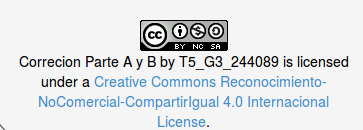
\includegraphics[width=10cm]{Licencia} \hspace{0.5cm}
\end{center}

\end{document}
